\documentclass[]{article}

\usepackage[utf8]{inputenc}
\usepackage[english,serbian]{babel}
\usepackage[margin=0.7in]{geometry}
\usepackage{url}
\usepackage{float}
\usepackage[graphicx]{realboxes}
\usepackage{listings}
\usepackage{textcomp}
\usepackage{xcolor}
\usepackage{titlesec}
\usepackage{adjustbox}
\lstset {
    language=HTML,
    frame=none,
    %xleftmargin=-.25in,
    %xrightmargin=.25in
    framesep=10pt,
    tabsize=4,
    showstringspaces=false,
    upquote=true,
    commentstyle=\color{black},
    keywordstyle=\color{black},
    stringstyle=\color{black},
    basicstyle=\small\ttfamily,
    emph={int,char,double,float,unsigned,void,bool},
    emphstyle={\color{black}},
    escapechar=\&,
    classoffset=1,
    morekeywords={>,<,.,;,,,-,!,=,~},
    keywordstyle=\color{black},
    classoffset=0,
    breaklines=true
}
\pagenumbering{gobble}

\titlespacing\title{left spacing}{before spacing}{after spacing}[right]

\title{Ra\v{c}unarske mre\v{z}e 4R, Ispit - Septembar 1}
\date{03.09.2019.}

\begin{document}

\makeatletter
\begin{center}

{\fontsize{12pt}{14pt}\selectfont\bfseries\@title\par}
\@date
\vspace{5mm}

Pro\v{c}itati sve zadatke \textbf{pa\v{z}ljivo} pre rada - sve \v{s}to nije navedeno ne mora da se implementira! 

Na \texttt{Desktop}-u napraviti folder sa imenom u formatu \texttt{rm\_sept1\_Ime\_Prezime\_mrGGXXX} i u njega smestiti \texttt{Java} projekat sa resenjima zadataka u zasebnim paketima sa imenima \texttt{zad1}, \texttt{zad2} itd. 

Vreme za rad: \textbf{2.5h}. Sre\'{c}no!
\end{center}
\makeatother


\begin{enumerate}
  \item Sockets and Channels \textbf{(15p)}
  \begin{itemize}
    \item Napraviti Java aplikaciju koja ima ulogu klijenta. Povezati se na lokalni server na portu 23456 koriste\'c{}i Java Sockets API i ispisuje podatke koje server \v{s}alje (server svake sekunde \v{s}alje trenutno vreme). Posle 5 uspe\v{s}nih primanja klijent prekida vezu (ili ako server prekine vezu pre vremena). \hfill (4p)
    \item Napraviti Java aplikaciju koja ima ulogu servera. Pokrenuti \textbf{neblokiraju\'c{}i} lokalni server na portu 23456 koriste\'c{}i Java Channels API. Server svim klijentima \textbf{jednom svake sekunde} \v{s}alje trenutno vreme u formatu \texttt{DD-MM-YYYY MM:SS}. Klijent ispisuje dobijeno vreme na standardni izlaz. O prekidu konekcije posle odredjenog broja slanja se stara klijent. \hfill (10p)
    \item Postarati se da su svi resursi ispravno zatvoreni u slu\v{c}aju izuzetka. \hfill (1p)
  \end{itemize}

  \item Swing \textbf{(15p)}
  \begin{itemize}
    \item Napraviti prozor i u njega dodati skrolabilnu komponentu za prikaz sadr\v{z}aja. Prikazani sadr\v{z}aj se inicijalno mo\v{z}e menjati. \hfill (1p)
    \item Dodati komponentu za unos URL-a koji vodi do HTML prezentacije (testirati na lokalnom fajl-sistemu koriste\'c{}i URL sa FILE protokolom). Dodati dugme \texttt{U\v{c}itaj} koje prikazuje izvorni kod prezentacije sa datog URL-a u komponenti za prikaz. Ako URL nije validan ili ne vodi do HTML fajla, ispisati odgovaraju\'c{}u poruku u komponenti za prikaz. \hfill (4p)
    \item Dodati dugme \texttt{Prikazi} \v{c}iji je efekat da u komponenti za prikaz HTML fajla vizuelno prika\v{z}e HTML prezentaciju \v{c}iji je izmenjeni izvorni kod uzet iz te iste komponente. Nakon aktivacije dugmeta ne mo\v{z}e se menjati sadr\v{z}aj komponente za prikaz \hfill (3p)
    \item Dodati dugme \texttt{Sacuvaj} \v{c}iji je efekat da sa\v{c}uva tekstualni sadr\v{z}aj iz komponente za prikaz na istoj putanji sa koje je pro\v{c}itan ulazni fajl. \hfill (3p)
    \item Ispo\v{s}tovati izgled aplikacije (ne me\v{s}ati redosled komponenti i postarati se da su odnosi u veli\v{c}ini kao na slici ispod). \hfill (2p)
    \item Omogu\'c{}iti da se prozor mo\v{z}e pro\v{s}iriti i smanjiti a da se raspored i razmera komponenti ne promeni. \hfill (2p)
  \end{itemize}

\end{enumerate}


\begin{figure}[H]
  \centering
  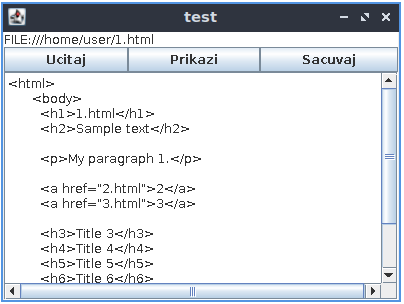
\includegraphics[scale=0.7]{fig1.PNG}
  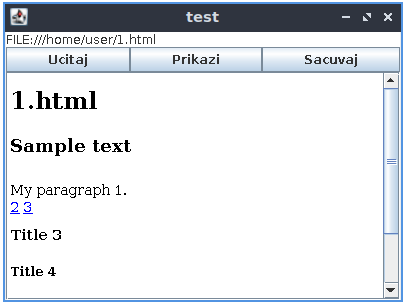
\includegraphics[scale=0.7]{fig2.PNG}
  \label{fig2}
  \caption{Izgled aplikacije pre i posle aktivacije dugmeta \texttt{Prikazi}}
\end{figure}


\newpage

HTML test fajlovi:\\

\noindent
\begin{tabular}{ccc}
\begin{lstlisting}
  <!DOCTYPE html>
  <html>
    <body>
      <h1>1.html</h1>
      <h2>Sample text</h2>
      
      <p>My paragraph 1.</p>

      <a href="2.html">2</a>
      <a href="3.html">3</a>

      <h3>Title 3</h3>
      <h4>Title 4</h4>
      <h5>Title 5</h5>
      <h6>Title 6</h6>

      Some text goes here.
    </body>
  </html>
\end{lstlisting}&
\begin{lstlisting}
  <!DOCTYPE html>
  <html>
    <body>
      <h1>2.html</h1>
      <h2>Sample text</h2>
      
      <p>My paragraph 2.</p>

      <a href="1.html">1</a>
      <a href="3.html">3</a>

      <h2>Title 2</h2>
      <h1>Title 1</h1>
      <h5>Title 5</h5>
      <h4>Title 4</h4>

      Text text text text.
    </body>
  </html>
\end{lstlisting}&
\begin{lstlisting}
  <!DOCTYPE html>
  <html>
    <body>
      <h1>3.html</h1>
      <h2>Sample text</h2>
      
      <p>My paragraph 3.</p>

      <a href="1.html" 
          id="1">1</a>
      <a href="2.html" 
          class="2">2</a>

      <h4>Title 4</h4>
      <h5>Title 5</h5>
      <h6>Title 6</h6>
      <h2>Title 2</h2>

      Text text text text.
    </body>
  </html>
\end{lstlisting}
\end{tabular} 

\end{document}
